\documentclass[a4paper]{article}
\usepackage{lmodern}
\usepackage{amssymb,amsmath}
\usepackage{ifxetex,ifluatex}
\usepackage{fixltx2e} % provides \textsubscript
\ifnum 0\ifxetex 1\fi\ifluatex 1\fi=0 % if pdftex
  \usepackage[T1]{fontenc}
  \usepackage[utf8]{inputenc}
\else % if luatex or xelatex
  \ifxetex
    \usepackage{mathspec}
  \else
    \usepackage{fontspec}
  \fi
  \defaultfontfeatures{Ligatures=TeX,Scale=MatchLowercase}
\fi
% use upquote if available, for straight quotes in verbatim environments
\IfFileExists{upquote.sty}{\usepackage{upquote}}{}
% use microtype if available
\IfFileExists{microtype.sty}{%
\usepackage{microtype}
\UseMicrotypeSet[protrusion]{basicmath} % disable protrusion for tt fonts
}{}
\usepackage[margin=1in]{geometry}
\usepackage{hyperref}
\hypersetup{unicode=true,
            pdftitle={Project 2},
            pdfauthor={Axel Sjöberg \& John Rapp Farnes},
            pdfborder={0 0 0},
            breaklinks=true}
\urlstyle{same}  % don't use monospace font for urls
\usepackage{longtable,booktabs}
\usepackage{graphicx,grffile}
\makeatletter
\def\maxwidth{\ifdim\Gin@nat@width>\linewidth\linewidth\else\Gin@nat@width\fi}
\def\maxheight{\ifdim\Gin@nat@height>\textheight\textheight\else\Gin@nat@height\fi}
\makeatother
% Scale images if necessary, so that they will not overflow the page
% margins by default, and it is still possible to overwrite the defaults
% using explicit options in \includegraphics[width, height, ...]{}
\setkeys{Gin}{width=\maxwidth,height=\maxheight,keepaspectratio}
\IfFileExists{parskip.sty}{%
\usepackage{parskip}
}{% else
\setlength{\parindent}{0pt}
\setlength{\parskip}{6pt plus 2pt minus 1pt}
}
\setlength{\emergencystretch}{3em}  % prevent overfull lines
\providecommand{\tightlist}{%
  \setlength{\itemsep}{0pt}\setlength{\parskip}{0pt}}
\setcounter{secnumdepth}{5}
% Redefines (sub)paragraphs to behave more like sections
\ifx\paragraph\undefined\else
\let\oldparagraph\paragraph
\renewcommand{\paragraph}[1]{\oldparagraph{#1}\mbox{}}
\fi
\ifx\subparagraph\undefined\else
\let\oldsubparagraph\subparagraph
\renewcommand{\subparagraph}[1]{\oldsubparagraph{#1}\mbox{}}
\fi

%%% Use protect on footnotes to avoid problems with footnotes in titles
\let\rmarkdownfootnote\footnote%
\def\footnote{\protect\rmarkdownfootnote}

%%% Change title format to be more compact
\usepackage{titling}

% Create subtitle command for use in maketitle
\providecommand{\subtitle}[1]{
  \posttitle{
    \begin{center}\large#1\end{center}
    }
}

\setlength{\droptitle}{-2em}

  \title{Project 2}
    \pretitle{\vspace{\droptitle}\centering\huge}
  \posttitle{\par}
    \author{Axel Sjöberg \& John Rapp Farnes}
    \preauthor{\centering\large\emph}
  \postauthor{\par}
      \predate{\centering\large\emph}
  \postdate{\par}
    \date{8 maj 2019}


\begin{document}
\maketitle

{
\setcounter{tocdepth}{3}
\tableofcontents
}
\newpage

\hypertarget{introduction}{%
\section{Introduction}\label{introduction}}

In this paper we bla bla

\hypertarget{analysis}{%
\section{Analysis}\label{analysis}}

\hypertarget{predicting-crime-rate-based-on-education-level}{%
\subsection{Predicting crime rate based on education
level}\label{predicting-crime-rate-based-on-education-level}}

\hypertarget{seeing-if-there-is-relationship}{%
\subsubsection{Seeing if there is
relationship}\label{seeing-if-there-is-relationship}}

We saw if there was a relationship by plotting bla bla with kernel
smoother.

\begin{figure}[h]
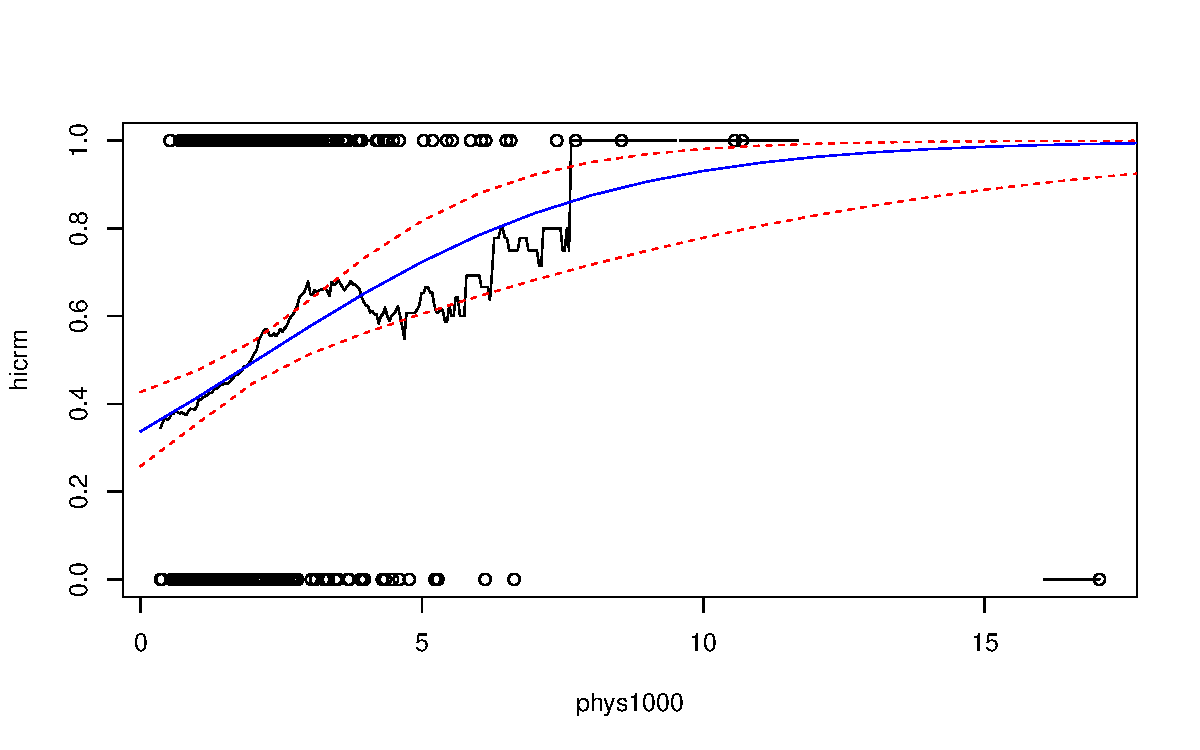
\includegraphics{Project_2_files/figure-latex/code_plot-1} \caption{Bla bla}\label{fig:code_plot}
\end{figure}

Seems to be relationship!

KOLLA UTAN BÖRJAN

--\textgreater{}

\hypertarget{confidence-intervals-and-significance}{%
\subsubsection{Confidence intervals and
significance}\label{confidence-intervals-and-significance}}

Report the beta-estimates together with their confidence intervals and
test whether the amount of adults with 12 years in school has a
significant effect on the probability of having a higher than median
crime rate

\begin{longtable}[]{@{}lrrrr@{}}
\caption{Test}\tabularnewline
\toprule
& Estimate & 2.5 \% & 97.5 \% & P-value (\%)\tabularnewline
\midrule
\endfirsthead
\toprule
& Estimate & 2.5 \% & 97.5 \% & P-value (\%)\tabularnewline
\midrule
\endhead
\(\beta_0\) & 3.866 & 1.527 & 6.27 & 0.044\tabularnewline
\(\beta_1\) & -0.050 & -0.081 & -0.02 & 0.041\tabularnewline
\bottomrule
\end{longtable}

Significance!

\hypertarget{change-in-odds}{%
\subsubsection{Change in odds}\label{change-in-odds}}

Estimate the relative change in the odds (odds ratio) of having a high
crime rate, with confidence interval, when the amount of higrads is
increased by 1 (percent), and when it is increased by 10 (percent).

If higrads increases 1\%, odd decreases by 4.9\% If higrads increases
10\%, odd decreases by 39.2\%

\hypertarget{predict}{%
\subsubsection{Predict}\label{predict}}

Use the model to predict the probability, with confidence interval, of
having a high crime rate in a county where the amount of higrads is 65
(percent), and where it is 85 (percent).

\begin{longtable}[]{@{}rrrr@{}}
\caption{Test}\tabularnewline
\toprule
Higrads & Probability & 2.5 \% & 97.5 \%\tabularnewline
\midrule
\endfirsthead
\toprule
Higrads & Probability & 2.5 \% & 97.5 \%\tabularnewline
\midrule
\endhead
65 & 0.6519376 & 0.5481793 & 0.7430377\tabularnewline
85 & 0.4087936 & 0.3415559 & 0.4796259\tabularnewline
\bottomrule
\end{longtable}

Use the model to predict, for each of the counties, whether it would be
expected to have a low or a high crime rate (predicted probability below
or above 0.5) and calculate the sensitivity and specificity for this
model.

Sensitivity is the proportion of the true successes that have been
correctly classified as successes (true positive). Specificity is the
proportion of the true failures that have been correctly classified as
failures (true negatives).

Sensitivity was 55\%

Specificity was 58.2\%

\hypertarget{predicting-crime-rate-based-on-region}{%
\subsection{Predicting crime rate based on
region}\label{predicting-crime-rate-based-on-region}}

Make a cross-tabulation between region and hicrm. Choose as reference
region in your regression models the one that has the largest number of
counties in it's smallest low/high category. As a tie-breaker, use the
other low/high category. Why is this a good idea? Hint: look at how the
standard errors for the log odds (ratios) are calculated in this
situation.

\begin{longtable}[]{@{}lrr@{}}
\caption{Test}\tabularnewline
\toprule
& Low crime & High crime\tabularnewline
\midrule
\endfirsthead
\toprule
& Low crime & High crime\tabularnewline
\midrule
\endhead
Northeast & 82 & 21\tabularnewline
Midwest & 64 & 44\tabularnewline
South & 44 & 108\tabularnewline
West & 30 & 47\tabularnewline
\bottomrule
\end{longtable}

Set the reference level to Northeast, makes sense to get low SE

Fit a logistic regression using region as (categorical) covariate and
report the beta-estimates together with their confidence intervals. Test
whether there are any significant differences between the regions in the
probability of having a high crime rate.

\begin{longtable}[]{@{}lrrrr@{}}
\caption{Test}\tabularnewline
\toprule
& Estimate & 2.5 \% & 97.5 \% & P-value (\%)\tabularnewline
\midrule
\endfirsthead
\toprule
& Estimate & 2.5 \% & 97.5 \% & P-value (\%)\tabularnewline
\midrule
\endhead
\(\beta_0\) & -1.362 & -1.867 & -0.903 & 0.000\tabularnewline
\(\beta_1\) & 0.988 & 0.383 & 1.616 & 0.162\tabularnewline
\(\beta_2\) & 2.260 & 1.682 & 2.874 & 0.000\tabularnewline
\(\beta_3\) & 1.811 & 1.162 & 2.492 & 0.000\tabularnewline
\bottomrule
\end{longtable}

Significant!

Estimate the odds ratios for having a high crime rate, with confidence
interval, for the different regions, compared to the reference region.

\begin{longtable}[]{@{}lrrr@{}}
\caption{Test}\tabularnewline
\toprule
& OR & 2.5 \% & 97.5 \%\tabularnewline
\midrule
\endfirsthead
\toprule
& OR & 2.5 \% & 97.5 \%\tabularnewline
\midrule
\endhead
South & 2.7 & 1.5 & 5.0\tabularnewline
Midwest & 9.6 & 5.4 & 17.7\tabularnewline
West & 6.1 & 3.2 & 12.1\tabularnewline
\bottomrule
\end{longtable}

Also estimate the probability of having a high crime rate, with
confidence interval, for the different regions, including the reference
region.

Calculate the sensitivity and specificity for this model. If we are
allowed to have either higrads or region as covariate, which one should
we choose?

\begin{longtable}[]{@{}lrrr@{}}
\caption{Test}\tabularnewline
\toprule
& Estimate & 2.5 \% & 97.5 \%\tabularnewline
\midrule
\endfirsthead
\toprule
& Estimate & 2.5 \% & 97.5 \%\tabularnewline
\midrule
\endhead
Northeast & 20.4 & 12.6 & 28.2\tabularnewline
Midwest & 40.7 & 31.5 & 50.0\tabularnewline
South & 71.1 & 63.8 & 78.3\tabularnewline
West & 61.0 & 50.1 & 71.9\tabularnewline
\bottomrule
\end{longtable}

Sensitivity was 70.5\%

Specificity was 66.4\%

\begin{longtable}[]{@{}lrr@{}}
\caption{Test}\tabularnewline
\toprule
Covariate & Sensitivity & Specificity\tabularnewline
\midrule
\endfirsthead
\toprule
Covariate & Sensitivity & Specificity\tabularnewline
\midrule
\endhead
Higrads & 0.55 & 0.58\tabularnewline
Region & 0.70 & 0.66\tabularnewline
\bottomrule
\end{longtable}

Would prefer region

\hypertarget{predicting-crime-rate-based-on-region-and-higrads}{%
\subsection{Predicting crime rate based on region and
higrads}\label{predicting-crime-rate-based-on-region-and-higrads}}

Fit a third model using both higrads and region. For all three models,
report their AIC, BIC, Nagelkerke pseudo R\^{}2, sensitivity and
specificity. Which model is best?

\begin{verbatim}
#> 
#> Call:
#> glm(formula = hicrm ~ higrads + region, family = "binomial", 
#>     data = cdi)
#> 
#> Deviance Residuals: 
#>      Min        1Q    Median        3Q       Max  
#> -1.96960  -0.99815  -0.04339   0.94402   1.94819  
#> 
#> Coefficients:
#>               Estimate Std. Error z value Pr(>|z|)    
#> (Intercept)    2.28073    1.28438   1.776 0.075774 .  
#> higrads       -0.04725    0.01645  -2.873 0.004069 ** 
#> regionMidwest  1.08760    0.31806   3.420 0.000627 ***
#> regionSouth    2.19684    0.30551   7.191 6.45e-13 ***
#> regionWest     1.95120    0.34749   5.615 1.96e-08 ***
#> ---
#> Signif. codes:  0 '***' 0.001 '**' 0.01 '*' 0.05 '.' 0.1 ' ' 1
#> 
#> (Dispersion parameter for binomial family taken to be 1)
#> 
#>     Null deviance: 609.97  on 439  degrees of freedom
#> Residual deviance: 527.32  on 435  degrees of freedom
#> AIC: 537.32
#> 
#> Number of Fisher Scoring iterations: 4
\end{verbatim}

\hypertarget{comparing-models}{%
\subsubsection{Comparing models}\label{comparing-models}}

\hypertarget{plot-skit}{%
\subsubsection{Plot \& skit}\label{plot-skit}}

Use the third model and plot the squared standardized Pearson residuals
and the standardized deviance residuals against the linear predictor
x\^{}beta. Is there anything alarming here? Plot Cook's distance against
the linear predictor, as well as against higrads and against region. Any
interesting finds?

\hypertarget{interaction}{%
\subsubsection{Interaction}\label{interaction}}

One might suspect that the effect of higrads is different in different
regions. Fit at fourth model adding the interaction higrads * region to
the third model, and use a Likelihood ratio test in order to determine
whether this is significantly better. Also calculate AIC, BIC,
Nagelkerke, sensitivity and specificity and plot the residuals and
Cook's distance. Do the interaction terms improve the model?

\hypertarget{other-variables}{%
\section{Other variables}\label{other-variables}}

Find a better model using combinations of the variables higrads, region,
poors and phys1000 = 1000*phys/popul (see Lab 3). You may ignore
interactions. Motivate why your model is better.


\end{document}
